\chapter{绪论}
\section{钛工业的发展历程与国内外现状}

钛(Titanium),原子序数为22,最早于1791年由格雷戈尔在英国康沃尔郡发现,是一种银白色的金属,具有密度小、比强度高、耐高温、化学性质性质稳定等明显优于传统金属的特性而备受重视。钛及钛合金常用来制造飞机、火箭等航天机械,一直以来都是航空航天工业的“脊柱”之一,被誉为“太空机械”\cite{XJYS200102014}。与纯钛一同发展起来的钛合金也毫不逊色,钛合金是在纯钛的基础上添加了各种各样的合金元素而形成的合金,凭借其更高的强度、耐蚀性、抗高温性能,得到了广泛的应用,尤其是在机械制造、航空航天、化工、军工等领域,钛合金的占比更大。钛工业的发展水平在一定程度上是衡量一个国家航空航天、汽车工业等领域发展水平的重要标志\cite{HSJJ202109005}。

\subsection{钛与钛合金的特点}
钛合金具有密度小,强度高的显著特点,相较于高强度钢而言,不仅强度相差无几,而且还具有更大的比强度。

\begin{table}[htbp]
	\centering
	\label{sec:bqd}
	\caption{不同合金比强度比较表}
	\begin{tabular}{ccccc}
		\toprule
		\textbf{合金} & \textbf{镁合金} & \textbf{铝合金} & \textbf{高强钢} & \textbf{钛合金} \\
		\midrule
		比强度 & 16 & 21 & 23 & 29 \\
		\bottomrule
	\end{tabular}
\end{table}

钛合金的特点如下\cite{1997titanium}:
\begin{enumerate}
	\item 熔点高。钛的熔点为1660℃,比铁的熔点还高出120℃左右。此外,在钛中加入铝、锆、锡等合金元素后,可以提高其热强性。
	\item 弹性模量低,屈服强度高,适合做弹簧材料。高端赛车内部的弹簧大多数都是由钛合金制成。
	\item 具有良好耐磨性、耐腐蚀性。钛表面易生成致密的氧化层,在氧化性或中性介质中有较强的耐腐蚀能力。
	\item 化学活性高。当钛加热到500℃以上时,氧化膜变得稀松且易脱落,在熔融状态下,极易发生自然。
	\item 特殊性能多。某些类型的钛合金还具有储氢、超导、低阻尼性,生物相容性、形状记忆 、 超弹 、高阻尼等特殊功能。
\end{enumerate}

\subsection{国外发展}
钛工业的发展充满曲折。从钛元素的发现(1791)到第一次制得较纯的金属钛(1910)经历了120年的历程。又由实验室第一次获得纯钛(1940)到首次进行工业生产,又花费了近30年的时间。
钛在自然界中主要以钛矿石的形式存在,如钛铁矿、金红石(TiO2)等,需要进行精炼(refining)才能获得纯金属。起初,钛的提取是通过高温还原法,但这种方法费时费力,成本高昂。直到了二十世纪四十年代,一种利用氯化钛矿与氯气进行反应来制备四氯化钛,然后通过还原反应(比如Na、Mg等)来得到纯钛的精炼工艺方法终于以其低廉的成本、高效的回收率得到了广泛的商业化应用。

第二次世界大战之后,世界上许多国家都开始意识到钛工业的重要性,钛工业在数年间便迅速发展成为航空、航天、军事等领域的关键材料。1954年,美国成功研发出Ti-6Al-4V合金,该合金在耐热性、强度、塑性、韧性、耐蚀性和生物相容性等方面均达到较高水平,凭借性能上的优势,\ti 迅速成为钛工业的主要合金,现已占据全部用钛量的50%以上,甚至可以说,许多其他型号钛合金不过是Ti-6Al-4V的改良版而已\cite{COLO200102000}。

\subsection{国内发展}
我国的钛工业发展起源于20世纪50年代,在六七十年代,我国成为了全球第四个建立完整钛工业体系的国家。自21世纪以来我国钛工业进入高速发展阶段,产能与产量已经连续多年占据世界第一的位置,目前海绵钛产量占全球比重已经达到六成,钛加工材产量稳定增长,钛产品消费端需求旺盛\cite{JSTB202209001},无论是在生产还是在加工领域均保持在世界前列。2014年,浙江余杭高端钛材的研发投产,标志着中国彻底摆脱了对国外的依赖,填补了中国高端钛材的技术空白。\cite{TGYJ200405004}

目前,我国的钛产品消费正处于上升期,如工业、航空航天、海洋船舶和体育休闲等中高端领域的钛材料的需求量平均增长约20%,而医疗行业受疫情影响,需求有所减少,电力和制盐等行业仍有小幅增长,整体盈利水平也有所改善\cite{BJKY202204004}。
%--------------------
%-------------------
%------------------
%------------------
%------------------

此外,近年来计算机技术的发展也为钛工业带来了新的发展机遇。计算机模拟技术用于优化钛合金的生产工艺,显著提高了产品质量。邵一涛等人利用BP人工神经网络的方法,构建了TC17钛合金组织和性能之间的关系模型,解决了传统BP人工神经网络的过拟合问题,从而获得更高的预测精度\cite{BP};李淼泉等人对 TC6 合金叶片在等温锻造过程中初生$\alpha$晶粒尺寸的演变进行了数值模拟\cite{Moni},将有限元法与 Yada 微观组织模型结合起来,并给出了 TC6 合金叶片在等温锻造过程中初生$\alpha$相的分布和晶粒尺寸的变化。在未来,随着物联网、大数据、人工智能、AIGC等技术的不断发展,钛工业也将迎来更多新的机遇和挑战。
\subsection{应用领域}

\begin{itemize}
\item  在航空航天领域,大型客机的设计制造推进迅速,同时军用飞机也在不断更新换代,因此全球钛合金的需求量也在急速增长。
\item  在医疗健康领域,钛合金材料有着良好的生物相容性,可以降低人体对植入物的排斥反应和感染风险,因此广泛用于人工关节、牙科种植体和其他医疗设备的制造。
\item  在汽车制造领域,高级车型的制造中广泛采用了钛合金零部件,以降低整车自重,提高燃油效率和汽车的运行性能。此外,钛合金耐腐蚀性好也能延长汽车零部件的使用寿命。
\item  在建筑工程领域,钛合金广泛应用于大型建筑的外墙幕墙、顶棚和立面系统中。这种材料具有优秀的耐候和抗腐蚀性能,可抵御各种恶劣气候的侵蚀,并且具有高度的可塑性和装饰性,可以为建筑带来更加优美的外观效果。

\end{itemize}
\section{钛合金的分类}
\label{sec:1.1}
因为纯钛的强度较低,限制了其在工业生产中的应用范围。钛合金是通过在纯钛中添加一些合金元素来提高其强度、耐腐蚀性等性能而形成的。常用的合金元素有铝、钒、锆、锂、铁、铜、镍等,通过调整元素配比和控制制备工艺,可以获得适合不同领域应用的各种高性能钛合金材料。

工业钛合金的主要合金元素为铝、钒、钼三种,此外还有Cr、Mn、Fe、Cu、Sn、Zr、W等元素组成,可以根据合金元素对钛多晶型转变温度的影响可将其分为三大类:$\alpha$稳定元素、$\beta$ 稳定元素、中性元素,形成的四种类型的相图示意图如图1.1所示。
\begin{figure}[h!]
	\centering
	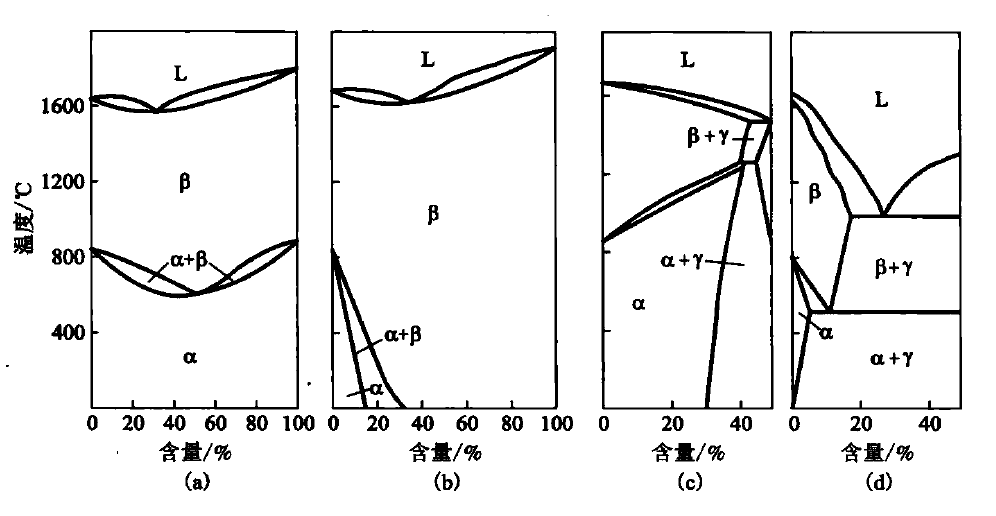
\includegraphics[width=0.9\linewidth]{pic/01}
	\caption{合金元素对钛合金相图的影响示意图}
	\label{fig:01}
\end{figure}

工业上一般根据$\beta$相稳定元素系数$K_{\beta}$来划分不同的合金元素,$K_{\beta}$是指合金中各$\beta$稳定元素与各自的临界浓度的比制之和,即:
\begin{equation}
K_{\beta}=\frac{ C_{1} }{C_{k1}}+\frac{ C_{2} }{C_{k2}}+\frac{ C_{3} }{C_{k3}}+\cdots+\frac{ C_{n} }{C_{kn}}
\end{equation}
根据 $\beta$ 相稳定系数划分合金类型为:
\begin{enumerate}
	\item  $\alpha$ 型合金 $K_\beta$ 为 $0 \sim 0.07$
	\item 近 $\alpha$ 型合金 $K_\beta$ 为 $0.07 \sim 0.25$
	\item $\alpha+\beta$ 型合金 $K_\beta$ 为 $0.25 \sim 1.0$
	\item 近 $\beta$ 型合金 $K_\beta$ 为 $1.0 \sim 2.8$
	\item $\beta$ 型 合金 $K_\beta$ 为 > 2.8
\end{enumerate}
\paragraph{(1)$\alpha$型}
经退火处理后,$\alpha$型钛合金的组织通常存在单相的$\alpha$固溶体,或者以含微量金属化合物的$\alpha$固溶体的形式存在。其主要合金元素包括铝、锡、锆等$\alpha$稳定元素,以及钒、钼、铌等中性元素,各个元素都可以起到固溶强化的作用,因此这些元素都被广泛地应用于钛合金的制备中。

常用的$\alpha$型钛合金包括TA2(工业纯钛)、TA9(Ti-0.2Pb)、TA10(Ti-0.3Mo-0.8Ni)等。

$\alpha$型钛合金的$\beta$相转变温度较高,因而具有良好的热强性、高温稳定性。焊接性性能好,并在高温环境下具有极好的组织稳定性和抗蠕变性能,在低温环境下也依然保持良好的延展性,因而适合制作各种飞行器形状复杂的外层板材。但它对热处理和组织类型不敏感,故不能采用热处理的方式强化其组织\cite{TiandAl}。
\paragraph{(2)$\beta$型}
$\beta$型钛合金主要包含钒、钼、铌、钽等$\beta$相稳定元素,若在合金中加入少量的铝、锆、锡等元素,则可以提高$\beta$型钛合金的塑性,并且改善其热稳定性。这些合金元素的加入可以控制合金的相转变温度,使其具有更加优异的力学性能和高温耐久性。
常见的$\beta$型钛合金有TB2(Ti-5Mo-5V-8Cr-3Al)、TB6(Ti-10V-2Fe-3Al)、TB7(Ti-36Mo)等。

与$\alpha$型、$\alpha+\beta$型钛合金相比,$\beta$型钛合金的显微组织通常更粗大。该合金具有良好的冷成形、冷加工性能,较好的淬火态塑性以及可焊接性。但是,亚稳态$\beta$型钛合金的热稳定性较差。$\beta$型钛合金中含有较高的$\beta$稳定元素,主要分为稳定$\beta$型钛合金和亚稳定$\beta$型钛合金。稳定$\beta$型钛合金在平衡状态下全部由稳定的$\beta$相组成,经热处理后不易产生变化。
\paragraph{(3)$\alpha$+$\beta$型}
经过退火处理的$\alpha+\beta$型钛合金在室温下具有不同比例的$\alpha$和$\beta$相组织,其锻造和轧制等加工成型性能比$\alpha$型、$\beta$型钛合金更加优异。合金中除了含有定量的铝元素外,还含有少量的其他元素,可以通过适当的热处理方法对$\alpha+\beta$型钛合金进行组织强化。其强度和淬透性随着$\beta$相稳定元素含量的增加而提高。

最常用的$\alpha$+$\beta$型钛合金包括TC4、TC6、TC12等,其中TC4钛合金(等轴马氏体型两相合金)作为做早被应用的钛合金,该合金以其优越的性能占据了钛工业的大量市场,现在占到 Ti 合金总产量的 50$ \%  $, 占到全部Ti 合金加工件的95$ \% $ 。

从成分上来看,这类钛合金中的合金元素基本上是以铝为主要合金元素,$\beta$稳定化元素为辅助元素。这使得$\alpha$+$\beta$型钛合金组织变动的余地较为灵活,性能变动范围大,可以满足各种应用场合及工况要求\cite{TiandAl}。
\section{钛合金的显微组织}
钛合金的性能是由显微组织的形态决定的, 甚至组织上的细微差异有时都会得到迥然不同的力学性能表现,显微组织形态则与元素含量、加工方式和热处理方式等环节息息相关。钛合金的基本组织有两种:低温的$\alpha$相和高温$\beta$相,两者特点如\ref{sec:alphaandbeta}所示:

\begin{table}[htbp]
	\centering
	\caption{钛合金基本组织的对比}
	\label{sec:alphaandbeta}
	\begin{tabular}{ccc}
		\toprule
		 特点&$ \alpha $相&$ \beta $相\\ \midrule
		 结构类型 & 六方最密堆积结构(HCP) & 体心立方结构(BCC) \\
		 原子排列 & 沿c轴密排 & 八面体最紧堆积结构\\
		 密度 & 4.43g/cm³ & 4.51g/cm³ \\
		 成分 & Ti-6Al-4V、Ti-6Al-2Sn-4Zr-2Mo等 & Ti-12Mo-6Zr-2Fe等 \\
		 形成温度 & 900℃-1000℃ & 700℃-800℃ \\
 		 稳定温度 & <882.5℃ & 882.5℃熔点 \\
 		 变形难易 & 困难 & 容易 \\
 		 滑移系 & 四个 & 十二个 \\
		 成形能力 & 较差,易发生晶粒长大、裂纹 & 易于变形,加工性能较好 \\
		 机械性能 & 强度和延展性能较好 & 韧性与热强性好 \\
		 耐腐蚀性能 & 良好 & 较差,易于发生点蚀、坑蚀等 \\
		\bottomrule
	\end{tabular}
\end{table}

TC4合金在加热到$ \beta $相变点以上后完全$ \beta $相化,但由于TC4合金内$ \beta $相稳定元素较少,体心立方的高温$\beta$相几乎不可能随着冷却过程保留到室温。$\beta$相在冷却过程中发生多种固态相变,形成多种多样的组织:随着温度降低,$\alpha$相以片状形态从原始$\beta$晶界析出。这种片状组织主要由相互交错的类似于珠光体一般的片层$\alpha$相与片层$\beta$相构成,称之为$\beta$转变组织。若合金在$\alpha+\beta$两相区状态下受到足够大的塑性变形,片状组织会把塑性变形产生的能量通过再结晶球化的方式再利用,得到形状规则的等轴组织。

根据转化后$\alpha$相的不同形态,TC4($\alpha+\beta$型)钛合金的显微组织大致分为四类:魏氏组织(片层组织)、网篮组织、双态组织以及等轴组织。各个组织的基本特点如下:
\begin{figure}[h!]
	\centering
	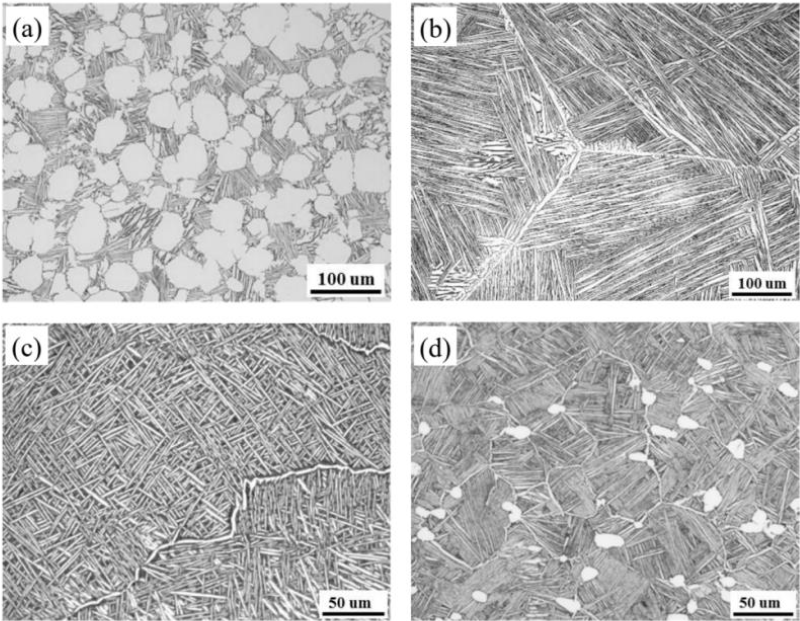
\includegraphics[width=0.7\linewidth]{pic/四种典型组织}
	\caption{四种典型组织(a)等轴组织;(b)魏氏组织;(c)网篮组织;(d) 双态组织}
	\label{fig:classic}
\end{figure}

\begin{itemize}
	\item 	\textbf{等轴组织}:在充分的塑性变形和再结晶退火后可以形成等轴组织。特点是$ \beta $基体上分布着等轴状的$ \alpha $相,疲劳强度高,具有良好的塑性,热稳定性。缺点是断裂韧性、持久强度差。
	\item 	\textbf{网篮组织}:合金在 $\alpha+\beta$ 两相区的塑性变形量不太大时形成网篮组织。其特点是晶内$ \alpha $片短小弯曲,在$ \beta $相晶粒周围分布,呈现出网篮状的形状,具有较高的疲劳强度和蠕变强度,塑韧性好。
	\item 	\textbf{双态组织}:双态组织与等轴组织类似,双态组织具有较高断裂韧性,疲劳裂性能好。等轴 $\alpha$ 含量在 $20 \%$ 左右的双态组织具有强度高、塑韧性好的综合力学性能,但高温性能较差。
	\item 	\textbf{魏氏组织}:在较高温度的 $\beta$ 区加热或变形量不够,时可以形成。如图\ref{fig:classic}(d)所示组织中 $\beta$ 晶粒的晶界比较完整,晶粒内有呈粗片状规则排列的长而平直的 $ \alpha $相,其断裂韧性、持久强度、蠕变性能好,但是塑性较差,疲劳强度低、热稳定性差,热处理时尽量避免该组织的形成。
\end{itemize}

\section{钛合金的相变}
钛合金的相变非常复杂,大体可以分为:同素异晶转变、共析转变、有序化转变、亚稳相分解、马氏体相分解等。

%	众多研究者已将钛合金的相变类型绘制成了一个表格:
%	\begin{table}[htbp]
	%	\centering
	%	\label{sec:change}
	%	\caption{相变过程}
	%		\begin{tabular}{ccc}
		%			\hline
		%			编号 & 相变 & 过程 \\ \hline
		%			I & 淬火过程中$\beta$相的分解 & (1)钛的马氏体:$ \beta $ 	o $\alpha^{\prime}$ , $\alpha^{\prime\prime}$\$ \\ \hline
		%	~ & 淬火过程中$\beta$相的分解 & (2)无热\$$\backslash$omega\$相:\$$\backslash$beta $\backslash$to $\backslash$omega\_\{$\backslash$text\{无热}} +$\backslash$beta\$ \\ \hline
%II & 等温转变中$\beta$相的分解 & (1) \$$\backslash$beta($\backslash$beta+$\backslash$alpha)$\backslash$to a\^\{\prime\prime},a\^\{\prime\prime}$\backslash$text\{富},a\^\{\prime\prime}$\backslash$text\{贫}\$ \\ \hline`
%~ & 等温转变中$\beta$相的分解 & (2) \$$\backslash$beta\^\{\prime}$\backslash$beta$\backslash$text\{富},$\backslash$beta$\backslash$text\{贫}\$ \\ \hline
%III & 残余$\beta$相分解 & (1)      相离析: \$$\backslash$beta\_\{$\backslash$text\{残}} $\backslash$to $\backslash$beta\^\{\prime}+$\backslash$beta\$ \\ \hline
%\end{tabular}
%\end{table}

在各种类型的钛合金中,$\beta$钛合金的用途最为广泛,在纷杂的钛合金相变中,可根据亚稳定状态相组成将其分为3类 :稳定$\beta$型钛合金 、 亚稳定$\beta$型钛合金和近$\beta$型钛合金。其中亚稳态$\beta$合金的综合性能最好,其相变过程也最复杂。亚稳定$\beta$相在快速冷却时,视合金成分不同,$ \beta $相可以转变成马氏体$ \alpha^{\prime} $或$ \alpha^{\prime\prime} $、$ \omega $或过冷$ \beta $相等亚稳定相。

通过快速冷却$\beta$相可以保持在亚稳定状态,但在一定温度下亚稳态会逐渐分解以降低系统的自由能。在温度不太高的情况下,由于密排六方点阵的$\alpha$相在体心立方点阵的$\beta$相基体中生核比较困难,所以不能直接分解形成平衡的$\alpha$相,需要经过一些中间分解过程,由生成的一些中间分解产物(或称过渡相)再转变为平衡的$\alpha$相。

依据钛合金的这种特性,可以根据不同的加热温度、冷却速度来进行处理以得到想要的微观组织,此即本设计采用固溶时效来强化合金性能的理论基础。
% 内容删减第一弹
%最常见的过渡相是等温相和$\beta$’相。在500℃范围内加热时,亚稳定$\beta$相的分解过程为:
%\begin{enumerate}
%	\item  $\beta$亚稳→$\beta$'+$\beta$→a\prime\prime+$\beta$→a+$\beta$
%	\item  $\beta$亚稳→$\beta$'+$\beta$→ω+$\beta$→a+$\beta$
%\end{enumerate}
%
%\subsection{马氏体相变}
% 钛合金自高温快速冷却时, 视合金成分不同, $\beta$ 相可转变为马氏体 ( $\alpha^{\prime}$ 或 $\left.\alpha^{\prime \prime}\right) 、 \omega$ 相或过冷 $\beta$ 相。在快速冷却过程中, 由于从 $\beta$ 相转变为 $\alpha$ 相的过程来不及进行, $\beta$ 相将转变为成分与母相相同、晶体结构不同的过饱和固溶体, 即马氏体。
%
%
% 我们知道马氏体转变是一种切变相变。在钛合金中发生马氏体转变时, $\beta$ 相中的原子作集体的有规律的近程迁移, 迁移距离较大时, 形成六方 $\alpha^{\prime}$ 相; 迁移距离较少时, 形成斜方 $\alpha^{\prime \prime}$ 。当 $\beta$ 相中的合金元素含量较少时, 原子位移较大, 点阵改组进行到底, 得到密排六方 $\boldsymbol{\alpha}^{\prime}$ 相; 当合金元素含量较大时, 点阵改组受到阻碍, 停留在某一中间阶段, 即形成斜方点阵 ( $\alpha^{\prime \prime}$ 相)。
%
%\subsection{ ω相变}
%合金成分在临界浓度$C_0$ 附近的合金从高温淬火后 , 将在合金组织中形成一种ω相。ω相可以根据组织分为两类——无热ω相与等温ω相。
%
%\begin{enumerate}
%	\item 无热ω相:当$\beta$合金元素的成分范围达到某一临界值时,合金在$\beta$相区淬火可以得到ω相。其特点是尺寸小,硬度大,脆性极大,会使材料的塑韧性急剧降低,当其含量达到80$ \% $时,合金就会失去宏观塑形。可以通过改变化学成分或者回火工艺予以控制。
%	\item 等温ω相:在淬火得到的亚稳定$\beta$相后,在随后的时效过程中,会出现$\omega \to \beta$转变,时效温度一般在100~500℃之间,相对于无热ω,$\beta$相分解为等温ω相的速度最快。其尺寸较小晶粒密度大,有方形和椭球形状两种形态,其含量越多,合金的硬度越高,塑韧性越差,当含量大约为50$ \% $时合金的综合性能较好。
%\end{enumerate}
%
%\subsection{$\alpha$相的形成}
% 在相分离和ω相变不能出现的高温时效过程中,亚稳$\beta$相可以直接转变为$\alpha$相,进而转变为$ 1\alpha $和$ 2\alpha $两种相
%
%%\begin{enumerate}
%%	\item  在位错及亚晶界上直接形成$\alpha$相;
%%	\item  经过过渡相形成a相
%%	\item  $\beta$→$\beta$'(bcc,贫溶质)→1$\alpha$和2$\alpha$;
%%	\item  $\beta$→ω(hcp,贫溶质)→l$\alpha$和2$\alpha$。
%%\end{enumerate}
%其中,1$\alpha$相为片层状,2$\alpha$为透镜状,但两者的晶体结构并无区别。
%在$\beta$相的时效转变中,有可能生成$\beta$'、ω、1$\alpha$和2$\alpha$相沉淀。$\beta$相对合金的强度无明显改善,相虽能强化合金,但会强烈降低合金的韧性。因此工业上的$\beta$合金都设计成使$\alpha$相(1$\alpha$和2$\alpha$)作为基体中的硬化沉淀相,合金的强度则由时效形成的$\alpha$相粒子尺寸、形状及体积分数控制。有实验数据表明,当合金中出现非共格的、有较大体积分数的、尺寸较大的2$\alpha$型沉淀时,合金将有良好的综合性能。


%\section{钛合金组织分析方法}

\section{\ti 合金研究进展}
近些年来国内对于\ti 合金的研究,主要在热处理工艺上取得了较多成果\cite{guokaiTC4taihejinrechuligongyideyanjiuxianzhuangjijinzhan2021}。

\begin{enumerate}
	\item 固溶处理:实施固溶处理工艺,是为了得到等轴稳定的$\alpha$相、马氏体弥散的$ \alpha^{\prime} $相、亚稳定状态的$\beta$相,等轴的$\alpha$相能够让合金的力学性能得到综合性的提升,马氏体弥散的$ \alpha^{\prime} $相能够让合金,在强度、硬度上得到提高,塑性、韧性被降低\cite{gurong2002}。
	\item 时效处理:有研究\cite{luyuanyuanShixiaochuliduiTC4taihejinweiguanzuzhihelixuexingnengdeyingxiang2019}发现,次生的$\alpha$相体积分数在TC4钛合金中,会对屈服强度产生很大的影响。在条件相等的情况之下,时效温度越低组织越小,时效温度高低组织越大。研究人员主要是通过控制参数,来影响对次生$\alpha$相的含量,从而来实现TC4钛合金在力学的性能上得到更好的提升。
	\item 深冷处理:深冷处理是近些年来新兴的一种处理工艺,其可以对金属内部的组织进行改善,在进行深冷处理的时候操作比较方便,对环境也不会造成太大的污染,并且能够让在热处理之后残留的奥氏体被清除掉。实验研究发现,原始的$\beta$相会在深冷处理的过程当中,逐渐的向$\alpha^{\prime}$相去转变,残余应力在组织中会变少,与此同时网篮状组织的增加,会让TC4钛合金的韧性、强度、塑性,在组织上的性能得到提高。
\end{enumerate}

\section{研究背景意义与研究内容}
\subsection{研究意义}
\ti 合金具有比强度高、生物相容性好、耐高温、化学性质性质稳定,等优良特性,在航空航天、汽车工业、医疗健康领域等领域得到了广泛应用,是目前应用最广泛的钛合金。但其室温塑性较低,加工硬化能力较差,冷加工成型困难。目前相关研究中,提升TC4钛合金室温塑性的手段主要包括\textbf{添加合金元素}、\textbf{剧烈塑性变形}和\textbf{相变热处理}。虽然前两种处理工艺对于合金的塑性提升明显,但工艺复杂、成本较高\cite{miao},而第三种热处理方法则工艺简单,成本较低,是提升TC4合金性能的不二之选。

钛合金的热处理方式属于共析和有序化转变,在退火和时效过程中存在共析 转变,时效过程中存在有序化转变,现阶段\ti 合金的基本热处理工艺主要有:深冷处理、固溶处理、渗氮处理等。不同的热处理工艺互相组合可以对合金产生更好的强化效果,现阶段工业上常采用\cite{zhoukaixiangJiyushenlengchulidenanjiagongcailiaoqiexiaotexingyanjiu2022}:淬火+时效;固溶+时效;双重固溶+时效;固溶+双重时效;时效+冷轧+低温氮化等,其中固溶+时效处理是应用最为广泛的一种热处理工艺组合。但是目前对于固溶+时效处理方法的最佳工艺参数一直没有定论,本设计的目的就是确定\ti 合金最佳的固溶+时效热处理工艺参数,并分析参数对于合金组织与力学性能的影响。

\subsection{研究内容}
本设计通过对TC4钛合金进行多种不同工艺参数的热处理,来重点研究不同固溶温度和冷却方式、时效的温度和时间下,TC4合金显微组织与力学性能的变化规律,重点关注$ \beta  $相稳定性变化及其对钛合金加工硬化和塑性的影响,以期为实际生产中探索高塑性TC4钛合金加工工艺提供理论依据。
设计的具体内容是:从\ti 合金板材中切取试样,采用\text{JC-MF12-30}型箱式电阻炉进行固溶与时效热处理;将热处理好的试样,放置在万能试验机上按{GB/T228-2002}进行室温力学性能测试,以得到合金的力学性能数值;然后对试样进行打磨抛光,在光学金相显微镜下进行组织的观察;最后分析工艺参数、力学性能与微观组织的关系,得到最佳热处理的工艺参数。
